% Player guide for "Leave at all costs". Build with:  pdflatex README.tex  (run it twice)
% and copy README.pdf to the repository root.
\documentclass[11pt, a4paper]{article}
\usepackage[margin=2.2cm]{geometry}
\usepackage[T1]{fontenc}
\usepackage{lmodern}
\usepackage{microtype}
\usepackage{xcolor}
\usepackage{booktabs}
\usepackage{tabularx}
\usepackage{enumitem}
\usepackage{tikz}
\usetikzlibrary{positioning, fit, backgrounds, calc, arrows.meta}
\usepackage[hidelinks]{hyperref}

\definecolor{alarm}{HTML}{C62828}
\newcommand{\cmd}[1]{\texttt{#1}}
\newcommand{\good}{\textcolor{green!45!black}{\textbf{good}}}
\newcommand{\bad}{\textcolor{alarm}{\textbf{bad}}}
\setlist{itemsep=2pt, topsep=4pt}

\title{\textbf{Leave at all costs}\\[2pt]\large A short text adventure about escaping a very boring class}
\author{Player guide}
\date{}

\begin{document}
\maketitle
\thispagestyle{empty}

\section*{The story}
You are in high school, sitting through the most boring Civics class of your life, and you
cannot take it any longer. After a few choices that may or may not end well for you, you find
yourself out in the school corridors. Unfortunately, the exit is locked. Use the items you find
and the people you meet to get out of school, \textcolor{alarm}{\textbf{AT ALL COSTS}}.

\section*{Goal}
There are \textbf{10 endings}, good and bad. Your goal is to reach all of them. A good ending
means you leave the school without any hiccups; everything else is a bad one. Each attempt
must be finished within \textbf{40 turns} --- run out of time and the principal catches you
(this does not count as an ending). Endings are remembered between attempts: after an
ending, choose \emph{Program $\to$ Try again} to play again.

The game rewards paying attention to details: read the location descriptions carefully.

\section*{Running the game}
\begin{itemize}
  \item You need Java 8 or newer. Double-click \texttt{At all costs (executable).jar}, or run
        \texttt{java -jar "At all costs (executable).jar"} in a terminal.
  \item \emph{Program $\to$ Map} opens the school map (\texttt{map.png}) in your image viewer.
        Keep \texttt{map.png} in the same folder as the \texttt{.jar} file.
        The map is also on page~\pageref{sec:map} of this guide.
\end{itemize}

\section*{How to play}
The game has two phases.
\begin{enumerate}
  \item \textbf{Multiple choice.} First type your name. After that, every turn gives you two
        options: answer \cmd{1} or \cmd{2}.
  \item \textbf{Adventure.} You walk around the school by typing commands:
\end{enumerate}

\begin{center}
\begin{tabularx}{0.9\textwidth}{@{}lX@{}}
  \toprule
  Command & What it does \\
  \midrule
  \cmd{go} \emph{direction}   & Move north, south, east, west, northeast, \dots, up or down. \\
  \cmd{get} \emph{item}       & Pick up an item you see. \\
  \cmd{drop} \emph{item}      & Put down an item you are carrying. \\
  \cmd{examine} \emph{item}   & Take a closer look at an item you are carrying. \\
  \cmd{use} \emph{item}       & Use an item you are carrying. \\
  \cmd{inventory}             & List what you are carrying. \\
  \cmd{ask}                   & Ask the person here for a favour. \\
  \cmd{rest}                  & Wait for a turn. \\
  \cmd{help}                  & Show the instructions. \\
  \cmd{endings}               & List the endings you have reached. \\
  \cmd{quit}                  & Give up this attempt. \\
  \bottomrule
\end{tabularx}
\end{center}

\noindent Some things to know:
\begin{itemize}
  \item \textbf{There are more commands than the ones listed.} They are single verbs hinted at
        in the location descriptions (sometimes you have to infer them!).
  \item Commands are not case-sensitive, and extra spaces are ignored.
  \item \cmd{help}, \cmd{endings} and commands the game does not understand do not use up a turn.
        Everything else does.
\end{itemize}

\section*{Endings}
\begin{center}
\begin{tabular}{@{}lll@{}}
  \toprule
  & Ending & Kind \\
  \midrule
  1  & Zzz\dots Zzz                   & \bad  \\
  2  & Humiliating!                   & \bad  \\
  3  & Stick to your lies!            & \bad  \\
  4  & Thank god for the nurse.       & \good \\
  5  & Lucky it ran on battery!       & \good \\
  6  & Dexterity 100!                 & \good \\
  7  & Certified pyromaniac           & \good? \\
  8  & A-Are you okay?                & \bad  \\
  9  & You already lied once\dots     & \bad  \\
  10 & Fool around and find out!      & \bad  \\
  \bottomrule
\end{tabular}
\end{center}

\noindent\textcolor{alarm}{\textbf{The school map is on the next page, the walkthrough on the last page.}}
Have a go before reading the walkthrough!

\newpage
\section*{School map}\label{sec:map}
North is up and east is to the right, matching the directions used in the game. Grey rooms
have stairs, so you can \cmd{go up} and/or \cmd{go down} from there.

\vspace{1em}
\begin{center}
  \resizebox{\textwidth}{!}{% The school map of "Leave at all costs", drawn with TikZ.
% This file only contains the picture; it is \input by map.tex (the standalone map that the
% game opens from its "Map" menu) and by README.tex.
%
% Required packages: tikz, with the libraries positioning, fit, backgrounds, calc, arrows.meta.
%
% Every room is placed on a grid so that the compass directions used in the game match the
% page: north is up, east is right. Grey rooms have stairs ("go up" / "go down").
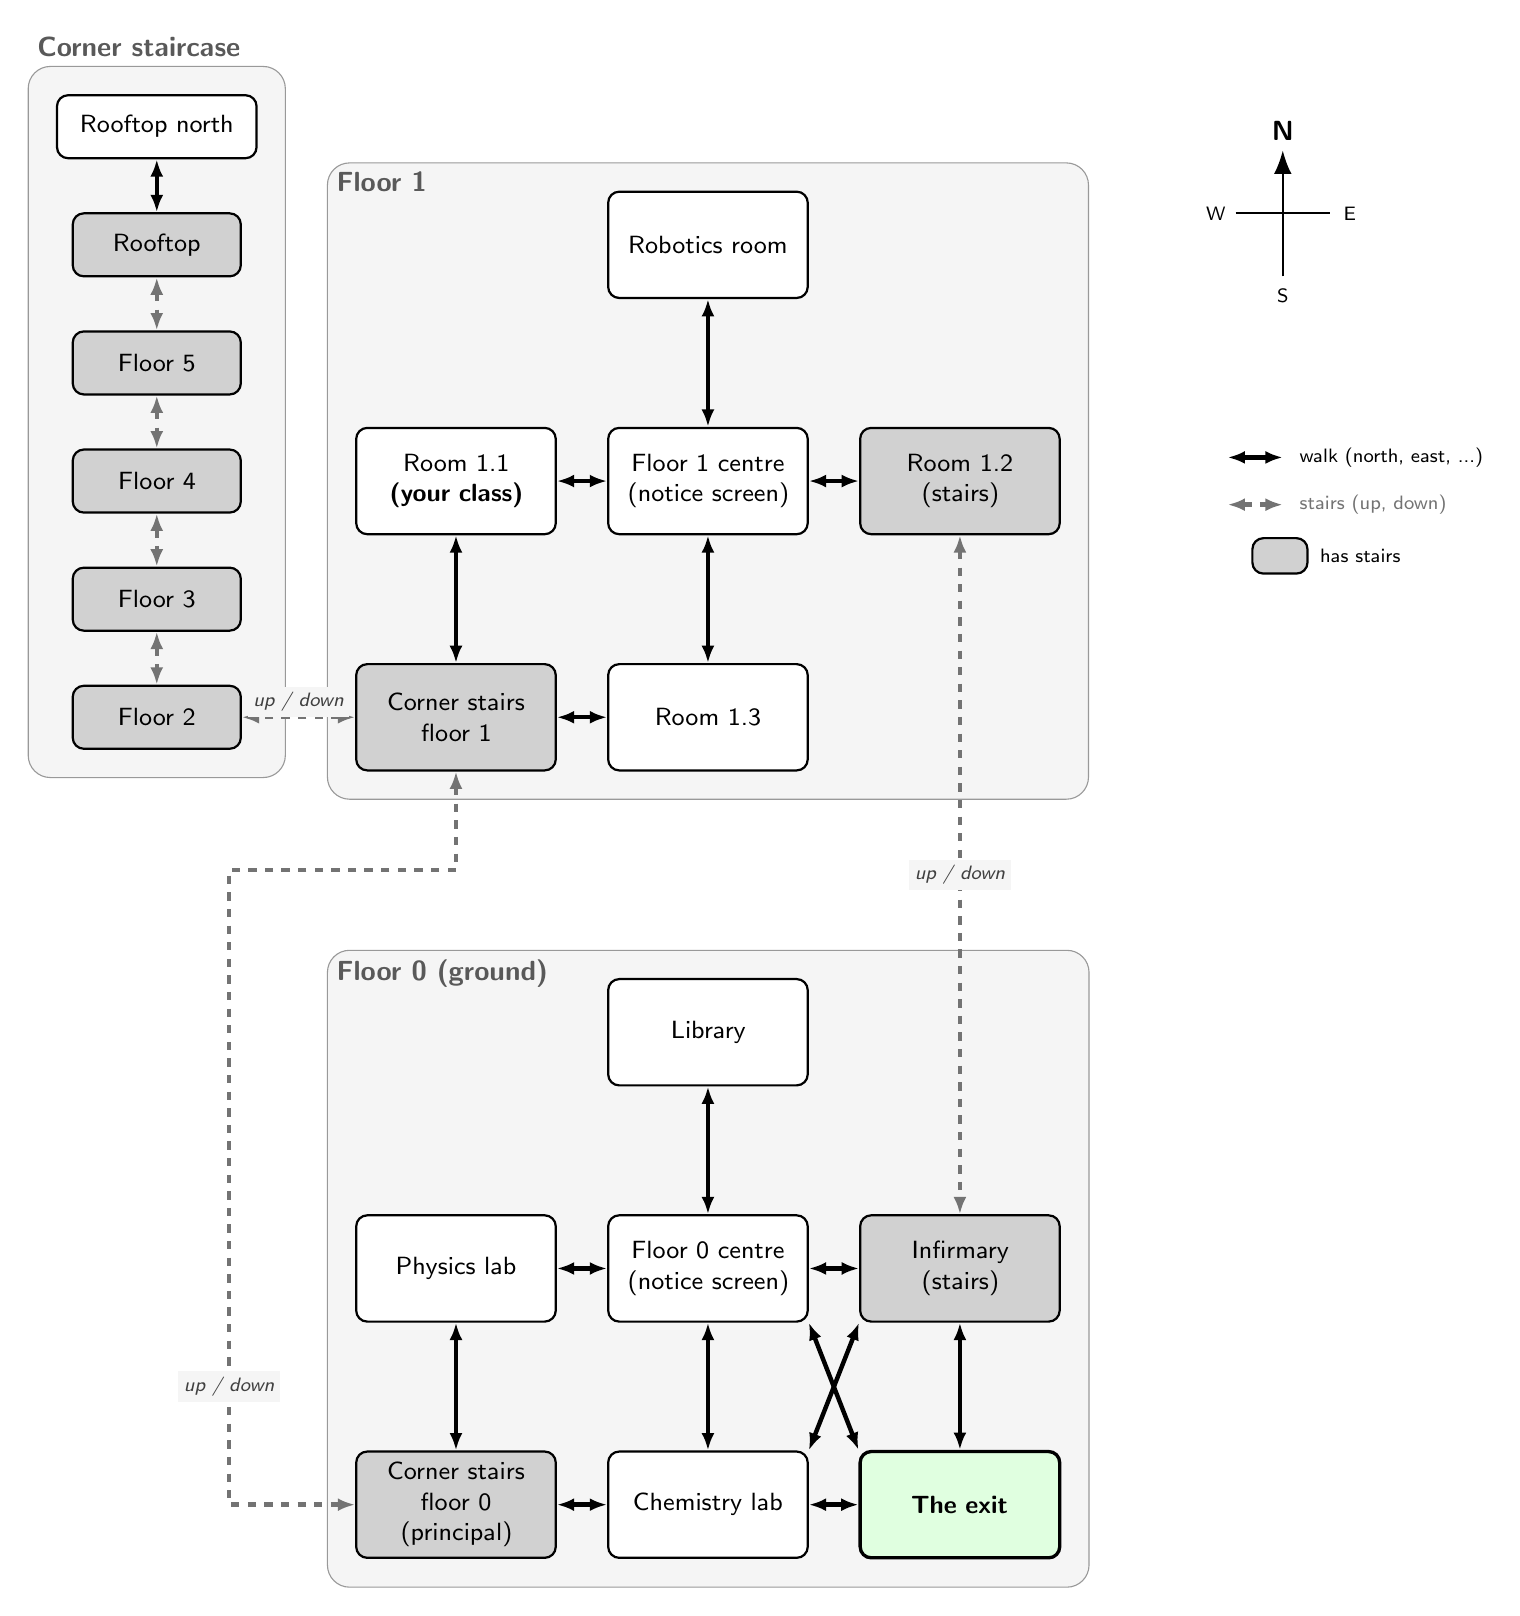
\begin{tikzpicture}[
    font=\sffamily\small,
    room/.style={draw, rounded corners=4pt, thick, fill=white, align=center,
                 minimum width=2.5cm, minimum height=1.35cm, text width=2.3cm},
    stairs/.style={room, fill=black!18},
    tower/.style={stairs, minimum width=2.1cm, minimum height=0.8cm, text width=1.9cm},
    link/.style={{Latex[length=2.2mm]}-{Latex[length=2.2mm]}, line width=1.6pt},
    vlink/.style={link, black!55, dashed},
    floor/.style={draw=black!40, fill=black!4, rounded corners=8pt, inner sep=10pt},
    floorlabel/.style={font=\sffamily\bfseries, anchor=north west, black!65},
    updown/.style={font=\sffamily\scriptsize\itshape, solid, draw=none, fill=black!4, text=black!75,
                   inner sep=2pt, line width=0pt},
  ]

  % ---------------- Floor 1 ----------------
  \node[room]   (robotics)  at (0, 3)   {Robotics room};
  \node[room]   (class)     at (-3.2, 0) {Room 1.1\\\textbf{(your class)}};
  \node[room]   (hall1)     at (0, 0)   {Floor 1 centre\\(notice screen)};
  \node[stairs] (room12)    at (3.2, 0) {Room 1.2\\(stairs)};
  \node[stairs] (corner1)   at (-3.2,-3) {Corner stairs\\floor 1};
  \node[room]   (room13)    at (0, -3)  {Room 1.3};

  % ---------------- Floor 0 ----------------
  \node[room]   (library)   at (0, -7)   {Library};
  \node[room]   (physics)   at (-3.2,-10) {Physics lab};
  \node[room]   (hall0)     at (0, -10)  {Floor 0 centre\\(notice screen)};
  \node[stairs] (infirmary) at (3.2,-10) {Infirmary\\(stairs)};
  \node[stairs] (principal) at (-3.2,-13) {Corner stairs\\floor 0\\(principal)};
  \node[room]   (chem)      at (0, -13)  {Chemistry lab};
  \node[room, very thick, fill=green!12] (exit) at (3.2,-13) {\textbf{The exit}};

  % ---------------- Stairs to the rooftop ----------------
  \node[tower] (s2)    at (-7, -3)   {Floor 2};
  \node[tower] (s3)    at (-7, -1.5) {Floor 3};
  \node[tower] (s4)    at (-7, 0)    {Floor 4};
  \node[tower] (s5)    at (-7, 1.5)  {Floor 5};
  \node[tower] (roof)  at (-7, 3)    {Rooftop};
  \node[room, minimum height=0.8cm] (roofN) at (-7, 4.5) {Rooftop north};

  % ---------------- Background panels ----------------
  \begin{scope}[on background layer]
    \node[floor, fit=(robotics)(class)(room12)(corner1)(room13)] (F1) {};
    \node[floor, fit=(library)(physics)(infirmary)(principal)(exit)] (F0) {};
    \node[floor, fit=(s2)(roofN)] (T) {};
  \end{scope}
  \node[floorlabel] at (F1.north west) {Floor 1};
  \node[floorlabel] at (F0.north west) {Floor 0 (ground)};
  \node[floorlabel, anchor=south west] at (T.north west) {Corner staircase};

  % ---------------- Same-floor connections ----------------
  \draw[link] (hall1) -- (robotics);
  \draw[link] (hall1) -- (class);
  \draw[link] (hall1) -- (room12);
  \draw[link] (hall1) -- (room13);
  \draw[link] (class) -- (corner1);
  \draw[link] (corner1) -- (room13);

  \draw[link] (hall0) -- (library);
  \draw[link] (hall0) -- (physics);
  \draw[link] (hall0) -- (infirmary);
  \draw[link] (hall0) -- (chem);
  \draw[link] (physics) -- (principal);
  \draw[link] (principal) -- (chem);
  \draw[link] (chem) -- (exit);
  \draw[link] (infirmary) -- (exit);
  \draw[link] (hall0.south east) -- (exit.north west);      % south-east
  \draw[link] (chem.north east) -- (infirmary.south west);  % north-east

  \draw[link] (roofN) -- (roof);
  \foreach \a/\b in {roof/s5, s5/s4, s4/s3, s3/s2} \draw[vlink] (\a) -- (\b);

  % ---------------- Stairs between floors (up / down) ----------------
  \draw[vlink] (room12) -- node[updown, pos=0.5] {up / down} (infirmary);
  \draw[vlink] (corner1.west) -- node[updown, above] {up / down} (s2.east);
  \draw[vlink] (corner1.south) -- ++(0,-1.25) -| ([xshift=-1.6cm]physics.west)
               |- node[updown, pos=0.25] {up / down} (principal.west);

  % ---------------- Legend and compass ----------------
  \begin{scope}[shift={(7.3, 3.4)}]
    \draw[thick, -{Latex[length=3mm]}] (0,-0.8) -- (0,0.8) node[above, font=\sffamily\bfseries] {N};
    \draw[thick] (-0.6,0) -- (0.6,0);
    \node[font=\sffamily\scriptsize] at (-0.85,0) {W};
    \node[font=\sffamily\scriptsize] at (0.85,0) {E};
    \node[font=\sffamily\scriptsize] at (0,-1.05) {S};
  \end{scope}
  \begin{scope}[shift={(7.3, -0.3)}, every node/.style={font=\sffamily\scriptsize, anchor=west}]
    \draw[link] (-0.7,0.6) -- (0,0.6) node[right=2pt] {walk (north, east, ...)};
    \draw[vlink] (-0.7,0) -- (0,0) node[right=2pt] {stairs (up, down)};
    \node[stairs, minimum width=0.7cm, minimum height=0.45cm, text width={}] at (-0.4,-0.65) {};
    \node at (0.35,-0.65) {has stairs};
  \end{scope}
\end{tikzpicture}
}
\end{center}

\newpage
\section*{Walkthrough \normalfont\small(spoilers!)}

\subsection*{Multiple-choice phase}
\begin{itemize}
  \item After you give your name, choosing to ignore the urge to sneak out makes you fall
        asleep in class $\to$ \bad\ ending \emph{Zzz\dots Zzz}.
  \item Otherwise you can \textbf{fake being ill} or \textbf{ask to go to the toilet}.
  \item Going to the toilet starts the adventure right outside your class (Room~1.1).
  \item If you fake being ill, you must let the teacher take you to the infirmary; refusing
        gives you away $\to$ \bad\ ending \emph{Humiliating!}
  \item The nurse asks what is wrong. You had been coughing and sniffling, so claiming a
        headache does not add up $\to$ \bad\ ending \emph{Stick to your lies!}
  \item Complaining about your breathing and throat works: the nurse gives you a sick note and
        the adventure starts at the infirmary.
\end{itemize}

\subsection*{Adventure phase: four ways to unlock the exit}
\begin{enumerate}
  \item \textbf{Sick note.} Get a sick note from the nurse (\cmd{ask} at the infirmary, unless
        you already have one) and \cmd{ask} the principal at the floor-0 corner stairs to unlock
        the exit $\to$ \good\ ending \emph{Thank god for the nurse.}
  \item \textbf{Prying.} Get the \emph{motor} from the robotics room and \cmd{ask} the physics lab
        instructor for a \emph{wrench}. At the exit, \cmd{use motor}, \cmd{use wrench} or
        \cmd{pry} $\to$ \good\ ending \emph{Lucky it ran on battery!}
  \item \textbf{Acid.} Get the \emph{black bottle} (sulphuric acid) from the chemistry lab and
        \cmd{use black bottle} at the exit $\to$ \good\ ending \emph{Dexterity 100!}
  \item \textbf{Fire.} Get the \emph{red canister} (fuel) from the floor-2 stairs and the black
        bottle, then go to the library and \cmd{use red canister}, \cmd{use black bottle} or
        \cmd{burn}. The fire alarm unlocks the exit $\to$ \good?\ ending \emph{Certified pyromaniac}.
\end{enumerate}
Only the first way you unlock the exit counts: once it is open, the other methods (and the
principal) will not work any more.

\subsection*{Accidents}
\begin{itemize}
  \item If you faked being ill, your teacher is watching the corridor. Spend 3 turns outside
        your class (Room~1.1) and they notice $\to$ \bad\ ending \emph{You already lied once\dots}
        (This cannot happen if you went ``to the toilet''.)
  \item After starting the fire, spend 2 more turns in the library, in one go or over several
        visits, and you pass out in the smoke. You are rescued, but arrested for arson
        $\to$ \bad\ ending \emph{Fool around and find out!}
  \item Climb the corner staircase all the way to the rooftop. The railing to the north is
        broken; from there \cmd{jump} or \cmd{go down} $\to$ \bad\ ending \emph{A-Are you okay?}
        This is meant to be the hardest ending to find: only a small hint in the text says you
        can jump.
\end{itemize}

\noindent Running out of turns (40) ends the attempt without unlocking an ending.

\vfill
\noindent\small\textcolor{black!60}{If you or someone you know is in a crisis, help is available.
Contact your local emergency number or a crisis helpline.}

\end{document}
